\documentclass{beamer}
\usecolortheme{beaver}
\usetheme{CambridgeUS}

\begin{document}
  \begin{frame}
    \frametitle{Background}
	\framesubtitle{Rendering hair}
	
	Important for variety of industries
	\begin{itemize}
	\item Animation movie industry: to render realistic hairs in a physically accurate way.
	\item Game industry: enhance realism and visual effects.
	\item Clothes manufacturing industry: to render custom fabrics and to compare appearance in different lighting conditions.
	\item Hair styling: render hair styling products applied to the hair.
	\end{itemize}
  \end{frame}
  
  \begin{frame}
    \frametitle{Rendering hair}
	\framesubtitle{Hair fiber representation}
	Explicit representation vs. Implicit representation
	
	\begin{itemize}
	\item Explicit representation represents each fiber by geometric primitives (e.g. triangles)
	\item Implicit representation represents fiber
	\end{itemize}
	
	There are a couple of ways to represent hair fibers:
	\begin{itemize}
	\item Connected triangle strips
	\item Cylindrical primitives
	\item Trigonal prisms
	\item Ribbons
	\end{itemize}
	

  \end{frame}
  
  \begin{frame}
    \frametitle{Rendering hair}
	\framesubtitle{Rendering challenges}
	
	Human hair consists of over hundreds of thousands of hair strands.
	Leads to rendering challenges:
	\begin{itemize}
	\item Memory consumption: to store all fibers in memory.
	\item Time: rendering realistic scattering effects requires tracing many samples through the hair volume.
	\item Aliasing: Hair fibers are very thin, requiring additional samples to be drawn to prevent aliasing.
	\end{itemize}
	

  \end{frame}
  
  % end Rendering hair
  
  \begin{frame}
    \frametitle{Mathematical notation}
	\framesubtitle{Radiometry}
	\begin{itemize}
	\item Power (Watts): energy in Joules per second.
	\item Radiant intensity (steradians): power divided by the solid angle.
	\item Irradiance (Watts per $m^2$): power per unit area.
	\item Radiance : Irradiance per solid angle, where solid angle goes to zero (becoming a ray instead of a cone).
	\end{itemize}
  \end{frame}
  
  \begin{frame}
    \frametitle{Mathematical notation}
	\framesubtitle{Scattering equations}
	
	Scattering is represented by a bidirectional reflection distribution function (BRDF):
	
	\begin{equation}
	f_r(p, \omega_o, \omega_i) = \frac{dL_o(p, \omega_o)}{dE(p, \omega_i)} = \frac{dL_o(p, \omega_o)}{L_i(p, \omega_i) \cos \theta_i d\omega_i}
	\end{equation}
	
	The BRDF is the fraction of outgoing radiance in direction $\omega_o$ related to the incident irradiance from direction $\omega_i$.

  \end{frame}
  
  \begin{frame}
    \frametitle{Mathematical notation}
	\framesubtitle{Hair fibers}
	
	
	
  \end{frame}
  
  
\begin{frame}
    \frametitle{Mathematical notation}
	\framesubtitle{Bidirectional curve scattering distribution function (BCSDF)}
	
	\begin{itemize}
	\item Hair fibers are rendered implicitly by 3D curves.
	\item Curves have no surface area. They have a length, requiring a change to the BRDF formulation.
	\end{itemize}
	
	\begin{equation}
	S_r(\omega_o, \omega_i) = \frac{dL_o(\omega_o)}{dE_i(\omega_i)} = \frac{dL_o(\omega_o)}{DL_i(\omega_i) \cos \theta_i d\omega_i}
	\end{equation}
	
	\begin{equation}
	L_o(\omega_o) = D \int S(\omega_i, \omega_o) L_i(\omega_i) \cos \theta_i d\omega_i
	\end{equation}

  \end{frame}  
  
  
% end mathematical notation  
  
  \begin{frame}
    \frametitle{Monte-Carlo integration}
    
    Numerical integration technique based on random numbers \\
    Possible to integrate any definite higher dimensional integrals.
    
    \begin{equation}
    F_N = \frac{b-a}{N} \sum^N_{i=1} f(X_i)
    \end{equation}
    
    \begin{equation}
    F_N = \frac{1}{N} \sum^N_{i=1} \frac{f(X_i)}{p(X_i)}
    \end{equation}
  \end{frame}
  
  \begin{frame}
    \frametitle{Multiple importance sampling}
  \end{frame}

	% end Importance sampling
  
  \begin{frame}
    \frametitle{Related work}
	\framesubtitle{Structure of hair}
	
	\begin{itemize}
	\item Hair fibers do have cuticle scales oriented at approximately 7 degrees.
	\item The core of the fiber (medulla and cortex) consist of pigment which absorbs specific wavelengths in the light.
	\end{itemize}
	
	\begin{figure}
	\includegraphics[scale=0.3]{../thesis/images/hair_structure.jpeg}
	\includegraphics[scale=0.25]{../thesis/hair-core.png}
	\end{figure}
  \end{frame}
  
  
  \begin{frame}
    \frametitle{Related work}
    \framesubtitle{Measured scattering data}
    Single fiber scattering model that models three visible scattering components:
    
    \begin{figure}
    \centering
    \includegraphics[scale=0.25]{../thesis/images/longitudinal_response.jpeg}
    \end{figure}
  \end{frame}
  
    \begin{frame}
    \frametitle{Related work}
    \framesubtitle{Marschner model}
    Single fiber scattering model that models three visible scattering components.
    \begin{itemize}
    \centering
    \item[R] reflection,
    \item[TT] double transmission,
    \item[TRT] transmission, reflection, transmission
    \end{itemize}
    
    \begin{columns}[onlytextwidth]
    \begin{column}{.45\textwidth}
    \begin{figure}
    	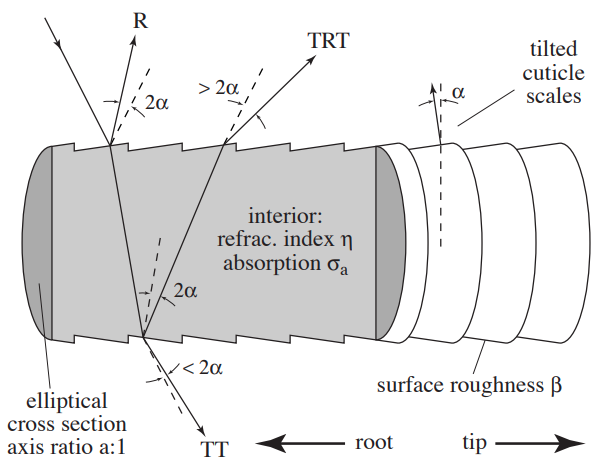
\includegraphics[scale=0.20]{../thesis/images/marschner_model_longitudinal.png}
    	\caption{Longitudinal scattering}
    \end{figure}
    \end{column}
    \hfill
    \begin{column}{.45\textwidth}
    \begin{figure}
    	\includegraphics[scale=0.09]{../thesis/circularcross.png}
    	\caption{Azimuthal scattering}
    \end{figure}
    \end{column}
    \end{columns}
  \end{frame}
  
  \begin{frame}
    \frametitle{Related work}
    \framesubtitle{Dualscattering Approximation}
  \end{frame}
  
  
  \begin{frame}
    \frametitle{Approach}
	Goals
  \end{frame}
  
  
  \begin{frame}
    \frametitle{Implementation}
    \framesubtitle{PBRT}
  \end{frame}
  
  \begin{frame}
    \frametitle{Implementation}
    \framesubtitle{Voxel grid}
  \end{frame}
  
  \begin{frame}
    \frametitle{Implementation}
    \framesubtitle{Memory and speed requirements}
  \end{frame}
  
  
  
  
  
  \begin{frame}
    \frametitle{Results}
  \end{frame}
  
  \begin{frame}
    \frametitle{Conclusion}
  \end{frame}
  
% etc
\end{document}